\chapter{Rotulação das imagens}

TEXTO AQUI.

\section{Mapas auto organizáveis}\label{sec:mapas_aut_organizaveis}

A maneira mais intuitiva de se agrupar imagens, ou qualquer outro tipo de
informação, é estabelecer um determinado número de classes e mapear cada imagem
para uma das classes, de modo que imagens semelhantes pertençam a mesma classe.
Entretanto, este tipo de abordagem desconsidera graus diferentes de semelhança
intra-classes, e até mesmo, graus diferentes de semelhança inter-classes, isto
é, havendo somente a ligação das imagens com suas classes como será possível
determinar, numericamente, o quão semelhante duas imagens são? Ou até mesmo,
quão diferentes são duas classes uma da outra?

Estas perguntas são relevantes porque, para os casos onde uma classe possui
centenas de imagens, muitas vezes o que se deseja é apenas uma amostra
significativa da classe, ou em outra situação, estando em pesse de uma
determinada imagem, deseja-se um número definido de imagens similares. Por isto,
um método voltado exclusivamente para agrupamentos pode não fornecer um conjunto
adequado de parâmetros que permitam extrair das classes informações como as
necessárias para responder as questões acima.

Partindo de um outro ponto, em vez de iniciar o projeto do \textit{clusterig} pelas
classes, mas sim pela distância entre as imagens, surge a possibilidade de criar
espaços para posicionar as imagens e, tendo a distância como medida de
diferença, definir as classes como regiões ou intervalos dentro destes espaços.
Deste modo, as classes não serão um parâmetro para a classificação, elas serão
definidas automaticamente pela dispersão das imagens nestes espaços através de
um processo dinâmico e automático. O resultado será não somente um método que
agrupa imagens mas que também define, sem a participação ativa do usuário, as
próprias classes utilizadas no agrupamento.

Estes espaços onde as imagens serão posicionadas podem ser de qualquer dimensão,
contudo, um espaço bidimensional de intervalos discreto é o suficiente para os
propósitos deste trabalho. Outro ponto importante é que estes espaços não podem
ser infinitos, pois obviamente estão limitados pela memória e pela capacidade
de processamento do computador, por isto, serão utilizados sempre espaços
limitados. Em resumo, podemos chamar estes subespaços bidimensionais discretos
de mapas, onde cada ponto é uma posição potencial para uma imagem, e as imagens
estão tão próximas quanto forem semelhantes.

Em resumo, a localização espacial de cada imagem e sua vizinhança topológica
representam, em um domínio ou característica particular, nestes casos os
momentos invariantes, uma classe, e estas classes são construídas de forma
emergente, sem nenhuma comparação com padrões desejados, por isto são ditos
auto organizáveis, como indica a Figura \ref{fig:mapa_classes_dist}.

\begin{figure}[H]
  \begin{center}
    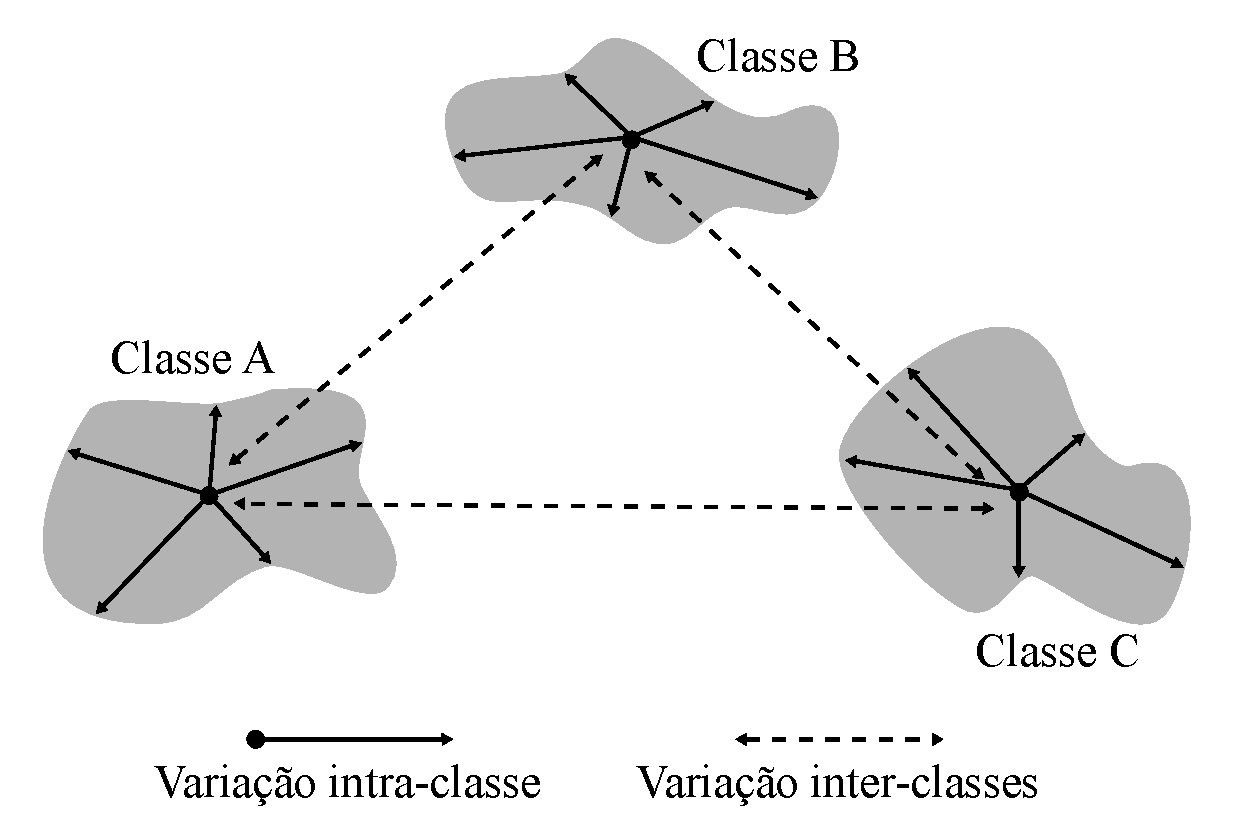
\includegraphics[height=6cm]{imagens/mapa_classes_dist.pdf}
  \end{center}
  \caption{ Organização das classes em um mapa auto organizável, coesão interna
    entre os elementos e isolamento externo entre as classes. }
  \label{fig:mapa_classes_dist}
\end{figure}

\section{Redes de Kohonen como mapa auto organizável}\label{sec:redes_kohonen_mapas}

Dentro da Inteligência artificial, mais especificamente no contexto do
aprendizado de máquina, as redes neurais artificiais são sistemas computacionais
inspirados na estrutura do cérebro, em particular dos neurônios, que adquirem
conhecimento através da experiência.

As redes neurais se assemelham a grafos direcionados, onde os nós são os
neurônios, ou unidades de processamento, que possuem uma quantidade indefinida
de conexões de entrada e saída. As conexões são o equivalente às arestas do
grafo, e são responsáveis por transmitir informações entre os neurônios, podendo
amplificar ou reduzir a acuidade destas informações. A Figura \ref{fig:neuronio}
apresenta o esquema típico de um neurônio.

\begin{figure}[H]
  \begin{center}
    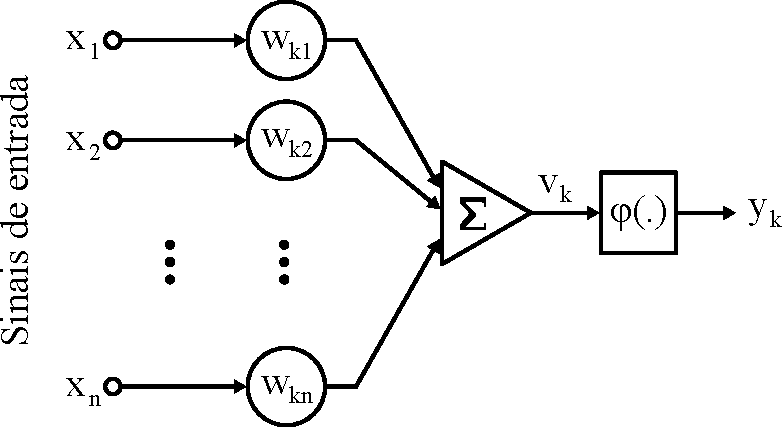
\includegraphics[height=4cm]{imagens/neuronio.pdf}
  \end{center}
  \caption{ Modelo de neurônio. }
  \label{fig:neuronio}
\end{figure}

Sinais de entrada provenientes de fora da rede chegam por meio de conexões
originadas do mundo externo, de modo semelhante, saídas da rede para o mundo
externo são conexões que deixam a rede.

A configuração da rede, ou seja, os peso atual das conexões, determina como os
dados de entrada irão ativar os diferentes neurônios e gerar um determinado
resultado. Para grande maioria dos tipos de redes neurais, uma configuração
particular é obtida através de um algoritmo de treinamento. O treinamento em
geral busca reforçar as conexões que geram bons resultados e penalizar as que
não geram.

As redes de Kohonen apresentam apenas duas camadas de neurônios, a camada de
entrada e a de saída. A camada de saída é uma espécie de malha de neurônios não
conectados entre si, mas amplamente conectados com os neurônios da camada de
entrada, como indicado na Figura \ref{fig:kohonen}. Esta malha funciona como um
mapa, onde para cada padrão de entrada
apenas um neurônio é ativado, padrões semelhantes ativam neurônios dentro de
uma mesma região da malha.

\begin{figure}[H]
  \begin{center}
    IMAGEM AQUI.
  \end{center}
  \caption{ Representação de uma rede de Kohonen. }
  \label{fig:kohonen}
\end{figure}

As redes de Kohonen possuem um algoritmo próprio de treinamento, dividido em
três etapas; na primeira, chamado de processo competitivo, uma determinada entrada
ativa apenas um neurônio da malha; na segunda, chamado de processo cooperativo,
o neurônio escolhido estabelece uma vizinhança de neurônios que serão ajustados
para, junto com ele, identificar padrões semelhantes ao que foi apresentado; e
por fim, na terceira etapa, chamada de processo adaptativo, os pesos são
atualizados com base no neurônio vencedor e na vizinhança topológica. Este
algoritmo de treinamento é dito não supervisionado, pois não depende de um
par \textit{(entrada, saída esperada)}, já que a própria rede estabelece como
será a configuração dos resultados, o processo de auto organização da rede.

\section{Características gerais de uma rede neural de Kohonen}\label{sec:caracteristicas_rede_kohonen}

Esta seção irá apresentar mais detalhadamente como é a configuração de uma rede
de Kohonen e seu algoritmo de treinamento.

\subsection{Topologia de uma rede de Kohonen}

Como dito anteriormente, a rede de Kohonen apresenta apenas duas camadas de
neurônios, a camada de entrada e a camada de saída. A camada de entrada deve
possuir tantos neurônios quanto forem à quantidade de elementos do padrão de
entrada. A camada de saída é uma grade de geometria livre, geralmente
retangular, de neurônios que não estão ligados entre si, mas estão, cada um,
ligados a todos os neurônios da camada de entrada. As conexões apresentam pesos
para escalar o sinal enviado. O esquema conceitual de uma rede de Kohonen é
demonstrado na Figura \ref{fig:kohonen_esquema}:

\begin{figure}[H]
  \begin{center}
    IMAGEM AQUI.
  \end{center}
  \caption{ Esquema detalhado de uma rede de Kohonen. }
  \label{fig:kohonen_esquema}
\end{figure}

\subsection{Treinamento da rede}

O treinamento requer que os pesos sinápticos sejam iniciados com valores bem
pequenos, para que a rede não apresente inicialmente nenhuma configuração. Três
processos são executados para cada entrada do conjunto de treinamento, o
processo competitivo, o processo cooperativo e o processo adaptativo.

\subsubsection{Processo competitivo}

Quando uma entrada $ x = \left[x_1, x_2, ..., x_n\right]^T $ é apresentado à
rede, o neurônio da grade que melhor responder a este padrão será ativado, este
neurônio é dito vencedor, e será recompensado ajustando-se seus componentes
para mais próximo do vetor de entrada.

O critério escolhido para determinar o neurônio vencedor é a distância
euclidiana entre o vetor de entradas e o vetor de pesos das sinapses do
neurônio, como indicado na equação \ref{eq:dit_ecl}:

\begin{equation}\label{eq:dit_ecl}
d_i(t) = \sqrt{\sum_{j = 1}^N \left( x_j(t) - w_{ij}(t) \right)^2}
\end{equation}

Onde:

\begin{itemize}
\item $ d_i(t) $ é a distância euclidiana entre o vetor de pesos do
neurônio $ i $ e o vetor de entradas na iteração $ t $;
\item $ i $ é o índice do neurônio da grade;
\item $ j $ é o índice do neurônio de entrada;
\item $ N $ é o número de entradas;
\item $ x_j(t) $ é o sinal de entrada na entrada $ j $ na iteração $ t $;
\item $ w_{ij}(t) $ é o valor do peso sináptico entre o neurônio de
entrada $ j $ e o neurônio da grade $ i $ na iteração $ t $.
\end{itemize}

\subsubsection{Processo cooperativo}

Estudos biológicos indicam que ao ser excitado, um neurônio estimula seus
vizinhos topológicos, de forma que quanto mais próximo um neurônio está do
neurônio ativo, mais excitado pelo estímulo do neurônio ativo ele é. O processo
cooperativo busca simular este mecanismo biológico.

Em termos matemáticos, o que se deseja é um parâmetro $ h_{ik} $ , dito
\textit{vizinhança topológica}, que indica o gral de cooperação entre o
neurônio vencedor $ i $ e o seu vizinho $ k $, que deve ser simétrico em relação
ao neurônio $ k $ e deve decrescer constantemente com o aumento da
distância $ l_{ik} $ , até que $ \lim\limits_{ l_{ik} \to \infty } h_{ik} = 0 $ .
A função gaussiana \ref{eq:gauss} atende a estas duas exigências:

\begin{equation}\label{eq:gauss}
h_{ik} = e^{ \left( \frac{ l_{ik}^2 }{ 2 \sigma^2 } \right) }
\end{equation}

O parâmetro $ \sigma $ é denominado \textit{largura efetiva da vizinhança},
e deve diminuir a cada iteração, indicando uma tendência de especialização da
rede. Neste trabalho o parâmetro $ \sigma $ é a equação \ref{eq:leg_eft}:

\begin{equation}\label{eq:leg_eft}
\sigma(t) = \sigma_0 e^{ t / \tau_l }
\end{equation}

Onde:

\begin{itemize}
\item $ \sigma_0 $ é o valor inicial de $ \sigma $;
\item $ t $ é a iteração atual;
\item $ \tau_l $ é uma constante de tempo.
\end{itemize}

\subsubsection{Processo adaptativo}

O processo adaptativo atualiza os pesos sinápticos a cada iteração, levando em
consideração o neurônio vencedor e a vizinhança topológica. O ajuste dos pesos
deve decrescer com o tempo, para evitar que novos dados comprometam seriamente
o conhecimento já adquirido, substituindo padrões já estabelecidos por novos.
Algo semelhante ocorre com o cérebro humano, ao decorrer do envelhecimento o
aprendizado vai se tornando mais difícil.

O ajuste $ \Delta w_{ij} $ que a sinapse entre o neurônio de entrada $ i $ e
um neurônio da malha $ j $ deve sofrer é expresso pela equação \ref{eq:ajus}:

\begin{equation}\label{eq:ajus}
\Delta w_{ij} = \eta(t) h_{ik}(t) (x_j - w_{ij})
\end{equation}

Onde $ h_{ik}(t) $ é o parâmetro vizinhança topológica na iteração $ t $ ,
referente ao neurônio vencedor $ k $ . O
parâmetro \textit{taxa de aprendizagem} $ \eta(t) $ é definido pela
expressão \ref{eq:tx_aprd}:

\begin{equation}\label{eq:tx_aprd}
  \eta(t) = \eta_0 e^{ t / \tau_l }, \eta_0 \in [0, 1]
\end{equation}

Onde $ \tau_l $ é uma constante de tempo.

\subsubsection{Algoritmo geral de treinamento}

O algoritmo \ref{alg:trei_khn} resume as três etapas anteriores e descreve
todo o processo de treinamento de uma rede de Kohonen:
%\clearpage

\begin{algorithm}[H]
\caption{Treinamento de uma rede de Kohonen}\label{alg:trei_khn}
\SetAlgoRefName{alg:trei_khn}
\Entrada{$ \sigma_0 $ , $ \tau_l $ , $ \eta_0 $ e o valor do \textit{erro} }
\Inicio{
  \Repita{distâncias auclidianas $ \le $ erro}{
    Calcular a \textit{largura efetiva} $ \sigma(t) $\;
    Calcular a \textit{vizinhança topológica} $ h $\;
    Calcular a \textit{taxa de aprendizado} $ \eta(t) $\;
    \ParaCada{conexão}{
      Calcular $ \Delta w $\;
      Ajustar o arco\;
    }
  }
}
\end{algorithm}

\section{Normalização dos dados de entrada da rede}\label{sec:entrada_rede}

Neste ponto já deve estar claro que a entrada da rede será o conjunto dos sete
momentos invariantes. Os momentos serão utilizados tanto na etapa de treinamento
quanto na classificação das imagens propriamente dita. Contudo, da forma como os
momentos são calculados ainda é necessário que eles passem por uma normalização
com o propósito de equalizar os valores dos momentos segundo sua real
contribuição para caracterização das imagens, isto é, para cada um dos conjuntos
de momentos, sete no total, um ajuste é feito sobre cada valor conforme o gral de
variação dos dados, isto porque, se os valores de um conjunto são muito
parecidos, pode-se concluir que este conjunto não é uma característica forte
para distinguir as diferentes classes de imagens, então deve ter uma influência
menor na classificação que os demais com alta variação dos dados.

A normalização também ajusta a faixa dos valores dos momentos. Dado que os
valores geralmente são bem pequenos, a normalização amplifica proporcionalmente
todos eles e evita problemas envolvendo operações computacionais com números
muito próximos de zero.

Sendo $ M $ a matriz com os valores originais dos momentos, na forma:

\begin{equation}\label{eq:momentos_matriz}
  M = \left[
    \begin{array}{cccc}
        m_{11} & m_{12} & \hdots & m_{17} \\
        m_{21} & m_{22} & \hdots & m_{27} \\
        \vdots & \vdots & \ddots & \vdots \\
        m_{n1} & m_{n2} & \hdots & m_{n7} \\
    \end{array}
  \right]
\end{equation}

A tranformação $ N(M) $ que normaliza todos dos elementos de $ M $ é dada por:

\begin{equation}\label{eq:momentos_transformacao}
  N_{ij} = \frac{m_{ij} - \overline{H}_j}{\sigma_j}
\end{equation}

Onde:

\begin{itemize}
\item $ m_{ij} $ é o momento da linha $ i $ coluna $ j $ de $ M $;
\item $ \overline{H}_j $ é a média de todos os elementos da coluna $ j $ de $ M $;
\item $ \sigma_j $ é desvio padrão $ \sqrt{\frac{\sum_{i=1}^n (m_{ij} - \overline{H}_j)^2}{n - 1}} $
      dos elementos da coluna $ j $.
\end{itemize}

Por fim, cada linha da matriz $ M $ é enviada para rede tanto na etapa do treinamento
quanto para classificação da imagem.

\section{A rede neural de Kohonen e o agrupamento das imagens}\label{sec:rede_kohonen_imagens}

TEXTO AQUI.

\subsection{Matriz de distâncias unificadas}\label{sec:u_matriz}

Tendo executado o treinamento da rede de Kohonen, pode parecer que a distância
euclidiana entre os elementos mapeados é o único parâmetro para a identificação
das classes, contudo, existe também uma distância do vetor de entrada para cada
posição do mapa, isto implica que também há uma outra distância entre os
neurônios além da distância euclidiana, uma distância que representa o grau de
dificuldade de se classificar uma elemento, no caso as imagens, em outra posição
diferente da que naturalmente lhe seria atribuída. Isto faz muita diferença
porque, mesmo tendo as classes que serem formadas por elementos adjacentes, esta
não é condição suficiente para identificação dos grupos, é possível que
dois elementos próximos pertençam a duas classes distintas, para isto basta
que a dificuldade de se classificar um desses elementos na posição do outro seja
superior a um limite estipulado.

Fazendo uma análise visual destas considerações, seria como se o mapa possuísse
campos de atração, formando vales e picos, sendo os vales as classes e os picos
os seus limites, ou fronteiras, como indica a Figura \ref{fig:mapa_x_umatriz}.

\begin{figure}[H]
  \begin{center}
    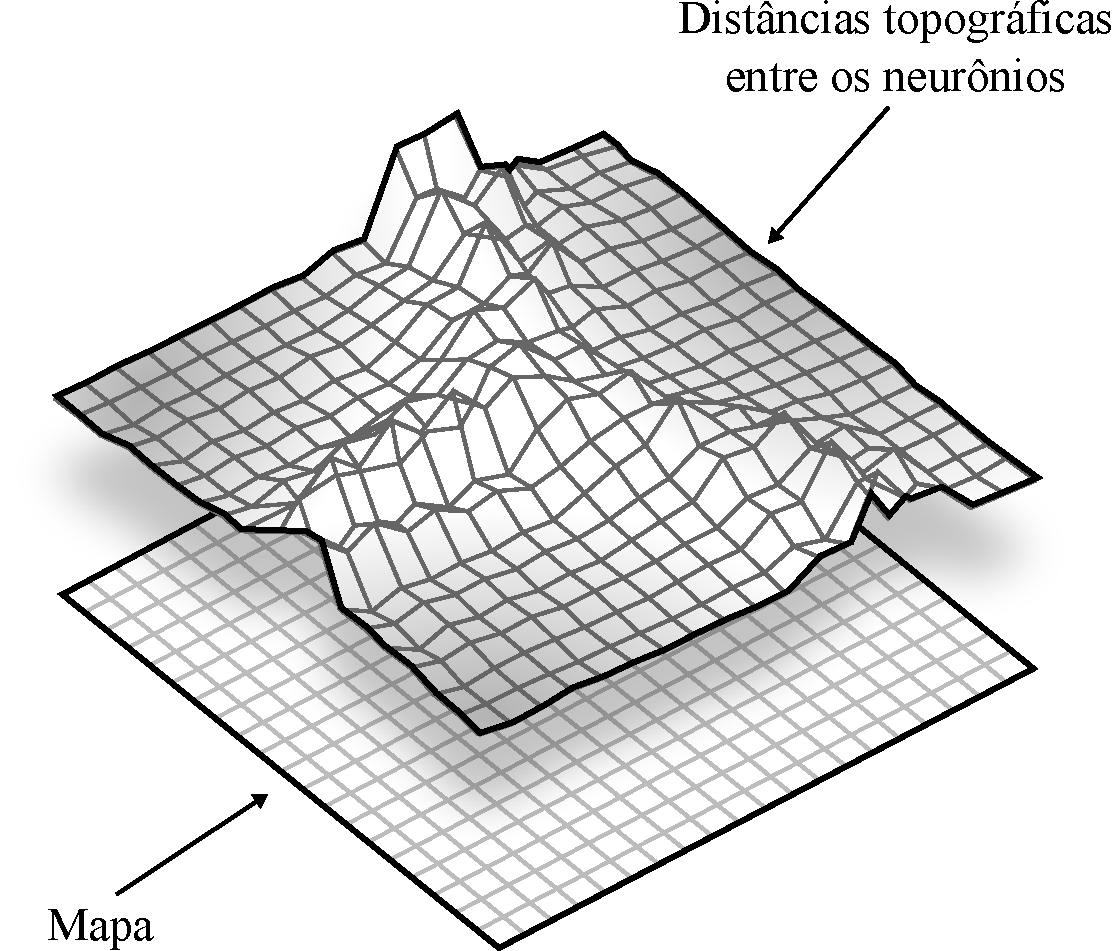
\includegraphics[height=8cm]{imagens/mapa_x_umatriz.pdf}
  \end{center}
  \caption{ Representação da malha de distâncias topográficas entre os neurônios }
  \label{fig:mapa_x_umatriz}
\end{figure}

O método denominado matriz de distâncias unificadas, ou simplesmente U-Matriz,
tem o objetivo de identificar estas relações topológicas, definindo uma função
tridimensional onde cada ponto do plano apresenta um valor de distância entre
neurônios adjacentes, de modo que valores baixos correspondem a neurônios
vizinhos semelhantes e valores altos correspondem a neurônios vizinhos
diferentes. Em termos matemáticos, regiões com baixos valores do gradiente,
vales, são classes de neurônios especializados em padrões similares e regiões
com valores altos correspondem a fronteiras entre as classes.

Considere o mapa retangular discreto limitado de tamanho $ N \times M $, para cada
neurônio $ p $ da camada de saída existe, na U-matriz, três distâncias, $ d_x $,
$ d_y $ e  $ d_{xy} $, em relação a seus vizinhos, como indicado na Figura \ref{fig:dxdydxy}.

\begin{figure}[H]
  \begin{center}
    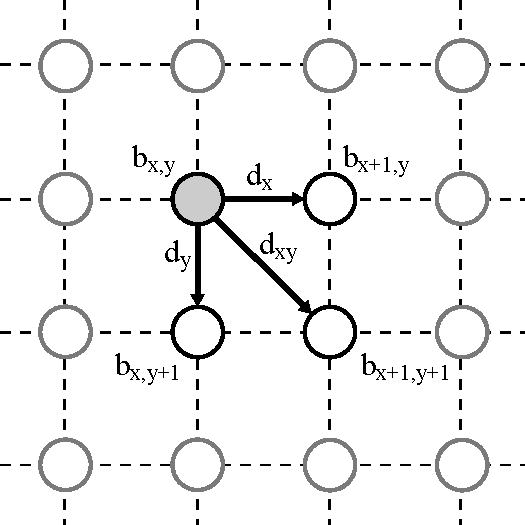
\includegraphics[height=6cm]{imagens/dxdydxy.pdf}
  \end{center}
  \caption{ Distâncias $ d_x $, $ d_y $ e $ d_{xy} $ entre o neurônio $ b_{x,y} $
    e seus visinhos. }
  \label{fig:dxdydxy}
\end{figure}

Os valores de $ d_x $, $ d_y $ e $ d_{xy} $ são calculados da seguinte maneira:

\begin{subequations}\label{eq:dxdydxy}
\begin{align}
  d_x(x, y) = \sqrt{\sum_i{ \left( w_{i(x,y)} - w_{i(x + 1, y)} \right)^2 }}\\
  d_y(x, y) = \sqrt{\sum_i{ \left( w_{i(x,y)} - w_{i(x, y + 1)} \right)^2 }}\\
  d_y(x, y) = \frac{1}{2\sqrt{2}}\sqrt{\sum_i{ \left( w_{i(x,y)} - w_{i(x + 1, y + 1)} \right)^2 } + \sum_i{ \left( w_{i(x,y + 1)} - w_{i(x + 1, y)} \right)^2 } }
\end{align}
\end{subequations}

Estes valores são inseridos em uma matriz de tamanho $ (N-1) \times (M-1) $ de acordo
com a seguinte tabela:

\begin{center}
\begin{tabular}{|c|c|c|}
\hline
  \textbf{i} & \textbf{j} & \textbf{$ U_{ij} $} \\
\hline
\hline
  $ 2x + 1 $ &     $ 2y $ & $ d_x(x,y) $    \\
\hline
      $ 2x $ & $ 2y + 1 $ & $ d_y(x,y) $    \\
\hline
  $ 2x + 1 $ & $ 2y + 1 $ & $ d_{xy}(x,y) $ \\
\hline
      $ 2x $ &     $ 2y $ & $ d_u(x,y) $    \\
\hline
\end{tabular}
\end{center}

Sendo $ c = [c_1, c_2, ..., c_k ] $ o vetor ordenado de elementos circunvizinhos
com cardinalidade $ k $, ainda levando em consideração um mapa retangular, o
cálculo de $ d_u $ é obtido pela mediana dos valores circunvizinhos,
do seguinte modo:

\begin{equation}\label{eq:du}
  d_u(x,y) = \left\{
    \begin{array}{rc}
                          c_{(k + 1)/2}, & \mbox{se $ k $ for ímpar} \\
      \frac{c_{k/2} + c_{(k + 1)/2}}{2}, & \mbox{se $ k $ for par}
    \end{array}
  \right.
\end{equation}

Deste modo, a organização da U-Matriz é ilustrada pela
Figura \ref{fig:mapa_umatriz}:

\begin{figure}[H]
  \begin{center}
    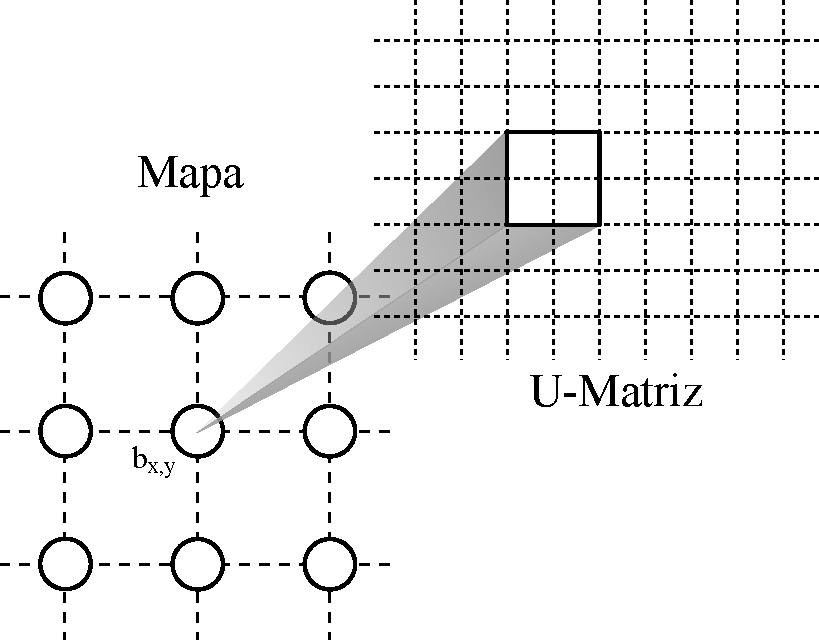
\includegraphics[height=6cm]{imagens/mapa_umatriz.pdf}
  \end{center}
  \caption{ Organização da U-Matriz em relação a grade de neurônios. }
  \label{fig:mapa_umatriz}
\end{figure}

\subsection{Transformada \textit{watershed} para rotulação automática
da U-Matriz}\label{sec:watershed}

A transformada de \textit{watershed} estabelece as regiões e fronteiras das
classes com base na U-matriz, faz isso apoiada no conceito intuitivo de
inundação, vales e diques, da seguinte maneira:

Como visto na Seção \ref{sec:u_matriz}, a U-matriz pode ser interpretada como
uma superfície que contem vales e montanhas, considerando uma inundação, a água
escorre pelas montanhas até os vales, que se inundam com o tempo, formando
bacias. Em um determinado momento certas bacias tenderão a se unir, esta união
é impedida pela "construção" de diques entre as regiões de fronteira. Ao fim do
processo, ou seja, quando a água chegar ao nível da maior montanha, os diques
formarão as fronteiras e as bacias formarão as classes. A Figura
\ref{fig:tempo_inundacao} Ilustra esse processo:

\begin{figure}[H]
  \begin{center}
    IMAGEM AQUI.
  \end{center}
  \caption{ Legenda. }
  \label{fig:tempo_inundacao}
\end{figure}

Uma definição formal da transformada de \textit{watershed} passa pela
consideração de dois períodos, isto é, pelo processo de expansão das bacias, em
outros termos, pela elevação de um nível $ h $ para $ h + 1 $.

Uma bacia associada a um mínimo $ m $ é denominada de $ B(m) $, os pontos dessa
bacia que possuem altitude menor ou igual a $ h $ são denominados $ B_h(m) $,
isto é:

\begin{equation}\label{eq:watershed_bm}
  B_h(m) = \{ p \in B(m) | f(p) \le h \}
\end{equation}

O subconjunto de todas as bacias que possuem pontos com altitude menor ou igual
a $ h $ é denominado $ X(h) $, formalmente:

\begin{equation}\label{eq:watershed_xh}
  X(h) = \bigcup_i B_h(m_i)
\end{equation}

Junto a esses conceitos fundamentais, o conjunto de todas os pontos que
pertencem ao mínimo regional $ m_h $ de elevação $ h $ é denominado $ R_{min_h}(f)$.
Esta região será definida posteiormente ainda nesta seção.

Considerando que os primeiros pontos a serem inundados são os pontos mínimos
$ h_{min} $, podemos aplicar a Equação \ref{eq:watershed_xh} da forma:

\begin{equation}\label{eq:watershed_xhmin}
  X(h_{min}) = R_{min_{h_{min}}}(f) = T_{h_{min}}(f)
\end{equation}

Onde $ T $ obedece a relação:

\begin{equation}\label{eq:watershed_t}
  T_h(f(x)) = \left\{
    \begin{array}{rc}
      x, & \mbox{se $ h \le f(x) $} \\
      0, & \mbox{qualquer outro}
    \end{array}
  \right.
\end{equation}

Utilizando $ h_{min} $ como ponto de partida, agora é necessário avançar para o
estágio onde o nível sobe uma unidade, ou seja, para $ h_{min + 1} $.
Neste ponto três situações podem ocorrer, isoladas ou simultaneamente, 1)
um novo mínimo será encontrado no ponto $ h_{min + 1} $ e formará uma
nova bacia, 2) ocorrerá uma expansão da bacia da região cujo mínimo é $ h_{min} $ e
3) duas ou mais bácias distintas de nível $ h_{min} $ estão se
expandindo e se encontrarão juntas. Estas três situações são ilustradas na
Figura \ref{fig:situacoes_inundacao}:

\begin{figure}[H]
  \begin{center}
    IMAGEM AQUI.
  \end{center}
  \caption{ Legenda. }
  \label{fig:situacoes_inundacao}
\end{figure}

1) $ Y_1 \cap X_{h_{min}} = \emptyset $: Nenhuma bacia foi formada, o que ocorrerá
apenas no próximo avanço de nível. Neste caso, vale a relação:

\begin{equation}\label{eq:watershed_caso1}
  \forall p \in Y_1 \left\{
    \begin{array}{rc}
      p \notin X_{h_{min}} \Rightarrow & f(p) \ge h_{min} + 1 \\
                 p \in Y_1 \Rightarrow & f(p) \le h_{max}
    \end{array}
  \right.
\end{equation}

2) $ Y_2 \cap X_{h_{min}} \neq \emptyset $ e é conectado: Neste caso a inundação já atingiu o
mínimo de $ Y_2 $ e o processo se encaminha numa expansão da bacia, o que pode
ser descrito como:

\begin{equation}\label{eq:watershed_caso21}
  Y_2 = B_{h_{min} + 1}(Y_2 \cap X_{h_{min}}) = Z_{Y_2}(Y_2 \cap X_{h_{min}})
\end{equation}

Onde $ Z_{Y_2}(Y_2 \cap X_{h_{min}}) $ é a zona de influência geodésica de
$ Y_2 \cap X_{h_{min}} $ contida em $ Y_2 $. Esta zona de influência
geodésica $ Z_A(K_i) $ de um componente conectado $ K_i $ dentro de um conjunto $ A $
é o lugar geométricos dos pontos
de $ A $ que a distância geodésica para $ K_i $ é a menor que a distância
geodésica para qualquer outro ponto de $ A $, em outros termos:

\begin{equation}\label{eq:watershed_caso22}
  Z_A(K_i) = \{ p \in A, \forall j \in [1, N] - \{ i \}, d_A(p, K_i) < d_A(p, K_j) \}
\end{equation}

Onde a distância geodésica $ d_A(p, q) $ entre dois pontos $ p $ e $ q $
pertencentes a $ A $ é o menor caminho entre todos os caminhos possíveis de
pontos, também pertencentes a $ A $, que ligam $ p $ e $ q $.

3) $ Y_3 \cap X_{h_{min}} \neq \emptyset $ e não é conectado: Neste caso $ Y_3 $
contém dois ou mais mínimos e eles estão expandindo juntos, denotados de
$ M_1, M_2, …, M_k $. Sendo $ M_i $ uma destas regiões a melhor aproximação
para $ B_{h_{min + 1}}(M_i) $ corresponde a zona de influência geodésica de $ M_i $
dentro de $ Y_3(M_Y)$:

\begin{equation}\label{eq:watershed_caso3}
  B_{h_{min + 1}}(M_i) = Z_Y(M_i)
\end{equation}

Como em 2) e 3) são bacias que estão em expansão, podemos definir estas regiões em termos
de uma única zona de influência geodésica $ X_{h_{min}} $, deste modo
$ X_{h_{min + 1}} $ é definido como a união destas zonas de influência geodésicas
onde os mínimos regionais foram os mais recentemente descobertos,
formulado em termos de uma recursão:

\begin{equation}\label{eq:watershed_recursao}
  \left\{
    \begin{array}{l}
      X_{h_{min}} = \bigcup_i h_{min_{i}} \in f \\
      X_{h + 1} = R_{min_{h + 1}}(f) \cup Z_{T_{t \le {h + 1}(f)}}(X_h)
    \end{array}
  \right.
\end{equation}

Por fim, o conjunto de bacias encontradas na U-matriz representam as classes e
servirão para rotular as imagens, para cada mínimo local haverá uma bacia e com
isso uma classe. Como o conjunto de mínimos locais pode ser grande, existe então
a chance de uma sobre segmentação da U-matriz, por isso é conveniente restringir
a quantidade de mínimos locais, no caso, os mínimos locais que geram bacias
com regiões muito pequenas, logo, é comum a utilização de filtros gaussianos
sobre a U-matriz antes de se aplicar a transformada de \textit{watershed} para
regularizá-la.

\section{Resumo do processo de classificação das imagens e do \textit{clustering}
como um todo}\label{sec:resumo_clustering}
